\documentclass[
%a4paper,12pt
encoding=utf8
]{./twoeskd}

% \usepackage{eskdappsheet}

% Packages required by doxygen
\usepackage[export]{adjustbox} % also loads graphicx
%\usepackage[draft]{graphicx}
\usepackage[utf8]{inputenc}
\usepackage{multicol}
\usepackage{multirow}
\usepackage{makeidx}

% NLS support packages
\usepackage[T2A]{fontenc}   
\usepackage[russian]{babel}
\usepackage{pscyr}

% Font selection
\usepackage{courier}
\usepackage{amssymb}

% Page & text layout
% \usepackage{geometry}
% \geometry{%
%   a4paper,%
%   top=2.5cm,%
%   bottom=4.5cm,%
%   left=2.5cm,%
%   right=2.5cm%
% }
%\setlength{\emergencystretch}{15pt}
\setlength{\parindent}{0cm}
\setlength{\parskip}{0.2cm}

% Headers & footers
% \usepackage{fancyhdr}
% \pagestyle{fancyplain}
% \fancyhead[L]{\fancyplain{}{}}
% \fancyhead[C]{\fancyplain{}{\scriptsize\textbf{RU.17701729.509000 ТЗ 01-1-ЛУ}}}
% \fancyhead[R]{\fancyplain{}{}}
% \fancyfoot[L]{\fancyplain{}{}}
% \fancyfoot[C]{\fancyplain{}{}}
% \fancyfoot[R]{\fancyplain{}{}}

% debug to see the frame borders
% from https://en.wikibooks.org/wiki/LaTeX/Page_Layout
% \usepackage{showframe}

% Indices & bibliography
\usepackage{natbib}
\usepackage[titles]{tocloft}
\setcounter{tocdepth}{3}
\setcounter{secnumdepth}{5}
\makeindex

% change style of titles in \section{}
\usepackage{titlesec}
\titleformat{\section}[hang]{\huge\bfseries\center}{\thetitle.}{1em}{}
\titleformat{\subsection}[hang]{\Large\normalfont\raggedright}{\thetitle.}{1em}{\underline}
\titleformat{\subsubsection}[hang]{\large\normalfont\raggedright}{\thetitle.}{1pt}{}

% Packages for text layout in normal mode
% \usepackage[parfill]{parskip} % автоматом делает пустые линии между параграфами, там где они есть в тексте
% \usepackage{indentfirst} % indent even in first paragraph
\usepackage{setspace}	 % controls space between lines
\setstretch{1} % space between lines
\setlength\parindent{0.9cm} % size of indent for every paragraph
\usepackage{csquotes}% превратить " " в красивые двойные кавычки
\MakeOuterQuote{"}


% this makes items spacing single-spaced in enumerations.
\newenvironment{my_enumerate}{
\begin{enumerate}
  \setlength{\itemsep}{1pt}
  \setlength{\parskip}{0pt}
  \setlength{\parsep}{0pt}}{\end{enumerate}
}


% Custom commands
% configure eskd
\titleTop{
\textbf{\Large ПРАВИТЕЛЬСТВО РОССИЙСКОЙ ФЕДЕРАЦИИ \\
НАЦИОНАЛЬНЫЙ ИССЛЕДОВАТЕЛЬСКИЙ УНИВЕРСИТЕТ \\
«ВЫСШАЯ ШКОЛА ЭКОНОМИКИ» } \\
\vspace*{0.2cm}
{\small Факультет компьютерных наук \\
Департамент программнoй инженерии \\
}
}
\titleDesignedBy{Студент группы БПИ 151 НИУ ВШЭ}{Куприянов К.И.}
\titleAgreedBy{%
\parbox[t]{7cm} {
Доцент департамента \\
программной инженерии \\
факультета компьютерных наук \\
канд. техн. наук \\
}}{Ахметсафина Р. З.}
\titleApprovedBy{
\parbox[t]{10cm} {
Академический руководитель \\
образовательной программы \\
«Программная инженерия» \\
профессор департамента программной \\
инженерии канд. техн. наук \\
}}{Шилов В. В.}
\titleName{Игра — Эскейп Квест с Использованием Очков Виртуальной Реальности}
\workTypeId{RU.17701729.509000 34 01-1}
\newcommand\tab[1][1cm]{\hspace*{#1}}
\titleSubname{Руководство оператора}

% Custom packages
\usepackage{pdfpages}

\makeindex

%===== C O N T E N T S =====


\begin{document}
% Titlepage & ToC
\pagenumbering{roman}

% some water filling text, that is pointless but adds text
% 
\tab[0.75cm] Техническое задание – это основной документ, оговаривающий набор требований и
порядок создания программного продукта, в соответствии с которым производится разработка
программы, ее тестирование и приемка.

Настоящее Техническое задание на разработку ``Клиент-Серверное Android-Приложение для Управления Скидками в Розничных Сетях'' содержит следующие разделы: ``Введение'', ``Основания для разработки'',
``Назначение разработки'', ``Требования к программе'', ``Требования к программным документам'',
``Технико-экономические показатели'', ``Стадии и этапы разработки'', ``Порядок контроля и
приемки'' и приложения.

В разделе ``Введение'' указано наименование и краткая характеристика области применения
``Клиент-Серверного Android-Приложения для Управления Скидками в Розничных Сетях''.

В разделе ``Основания для разработки'' указан документ на основании, которого ведется
разработка и наименование темы разработки.

В разделе ``Назначение разработки'' указано функциональное и эксплуатационное
назначение программного продукта.

Раздел ``Требования к программе'' содержит основные требования к функциональным
характеристикам, к надежности, к условиям эксплуатации, к составу и параметрам технических
средств, к информационной и программной совместимости, к маркировке и упаковке, к
транспортировке и хранению, а также специальные требования.

Раздел ``Требования к программным документам'' содержит предварительный состав
программной документации и специальные требования к ней.

Раздел ``Технико-экономические показатели'' содержит ориентировочную экономическую
эффективность, предполагаемую годовую потребность, экономические преимущества разработки
``Клиент-Серверного Android-Приложения для Управления Скидками в Розничных Сетях''.

Раздел ``Стадии и этапы разработки'' содержит стадии разработки, этапы и содержание
работ.

В разделе ``Порядок контроля и приемки'' указаны общие требования к приемке работы.

Настоящий документ разработан в соответствии с требованиями:\\
1) ГОСТ 19.101-77 Виды программ и программных документов \cite{gost_types_of_software};\\
2) ГОСТ 19.102-77 Стадии разработки \cite{gost_stages_of_devel};\\
3) ГОСТ 19.103-77 Обозначения программ и программных документов \cite{gost_marking_software};\\
4) ГОСТ 19.104-78 Основные надписи \cite{gost_main_signs};\\
5) ГОСТ 19.105-78 Требования к программным документам \cite{gost_demands_for_docs};\\
6) ГОСТ 19.201-78 Техническое задание. Требования к содержанию и оформлению \cite{gost_tz}.\\

Изменения к данному Техническому заданию оформляются согласно ГОСТ 19.603-78 \cite{gost_main_rules_change},
Перед прочтением данного документа рекомендуется ознакомиться с терминологией,
приведенной в Приложении 1 настоящего технического задания.


\newpage
\pagenumbering{arabic}
\tableofcontents
% \pagenumbering{arabic}

% --- add my custom headers ---
\newpage
\section{Назначение программы}
\subsection{Наименование программы}
Наименование программы на русском:
``Клиент-Серверное Android-Приложение для Управления Скидками в Розничных
Сетях''. \\
Наименование на английском:
``The Client-Server Android Application for Managing the Products' Discounts in
Retail Networks''.


\subsection{Краткая характеристика}
Программа предназначена для пользователей смартфонов на базе платформы Android.
Цель работы - создать удобное приложения для составления списков покупок,
добавления в них любых товаров (даже тех, которых нет в магазине), отслеживания
акций, а так же просмотра всех акций в нескольких магазинах. Это позволит
пользователям экономить свои средства на ежедневных покупках и быть в курсе
актуальных акций магазинов.  Серверная часть приложения должна представлять из
себя web-crawler для сбора данных с сайтов розничных сетей. Crawler должен
иметь модульную структуру, для быстрого восстановления после изменения дизайна
сайтов. Должен быть реализован механизм взаимодействия с клиентами посредством
обменивания файлами в формате JSON.\\
Главной чертой данного приложения
является его лёгкая, быстрая масштабируемость и модульность программного кода.



\newpage
\section{Условия использования программы}
%=========================================
\subsection{Минимальные параметры технических средств}
Для оптимальной работы приложения необходимо учесть следующие системные требования:
\begin{my_enumerate}
    \item Мобильный телефон со следующими минимальными требованиями:
    \begin{my_enumerate}
        \item Операционная система Android версии 4.4.4 KitKat и выше (API level 19+)
        \item 64-разрядный (x64) процессор
        \item 1ГБ оперативной памяти (ОЗУ)
        \item 100 МБ свободного места на внутреннем накопителе
    \end{my_enumerate}
    \item Наличие интернет-соединения со скоростью не меньше 30Мбит/c
\end{my_enumerate}


\subsection{Численность и калификация персонала}
Минимальное количество персонала, требуемого для работы программы: 1 оператор.
Пользователь данного программного продукта должен разбираться в работе
мобильных устройств, уметь устанавливать и удалять программы, запускать их.
Перед использованием программы пользователь должен заранее проинструктирован и
уведомлен о составе выполняемых функций и других характеристиках приложения.



\newpage
\section{Выполнение программы}
\subsection{Загрузка файлов}
В данном разделе будет показано, как устанавливать программу и пользоваться ей. Для описания каждого проделанного шага будут включены описание действий и скриншоты приложения.
\subsubsection{Установка программы}
Дистрибутив данной программы можно будет получить по ссылке, считав ее с
прилагаемого qr-кода(рис.~\ref{ref})

\begin{figure}[h!]
    \centering
    
\includegraphics[width=0.7\textwidth]{./screenshots/3/qr.png}
    \caption{ссылка на программу}
    \label{ref}
\end{figure}

Чтобы начать испытания выполнения требований к функциональным характеристикам,
необходимо запустить установщик программы путем нажатия на его иконку. После
запуска установщика появится приветственное окно мастера установки (рис.~\ref{install1},~\ref{install2},~\ref{install3}).

\begin{figure}[h!]
    \centering
    \minipage{0.3\textwidth}
    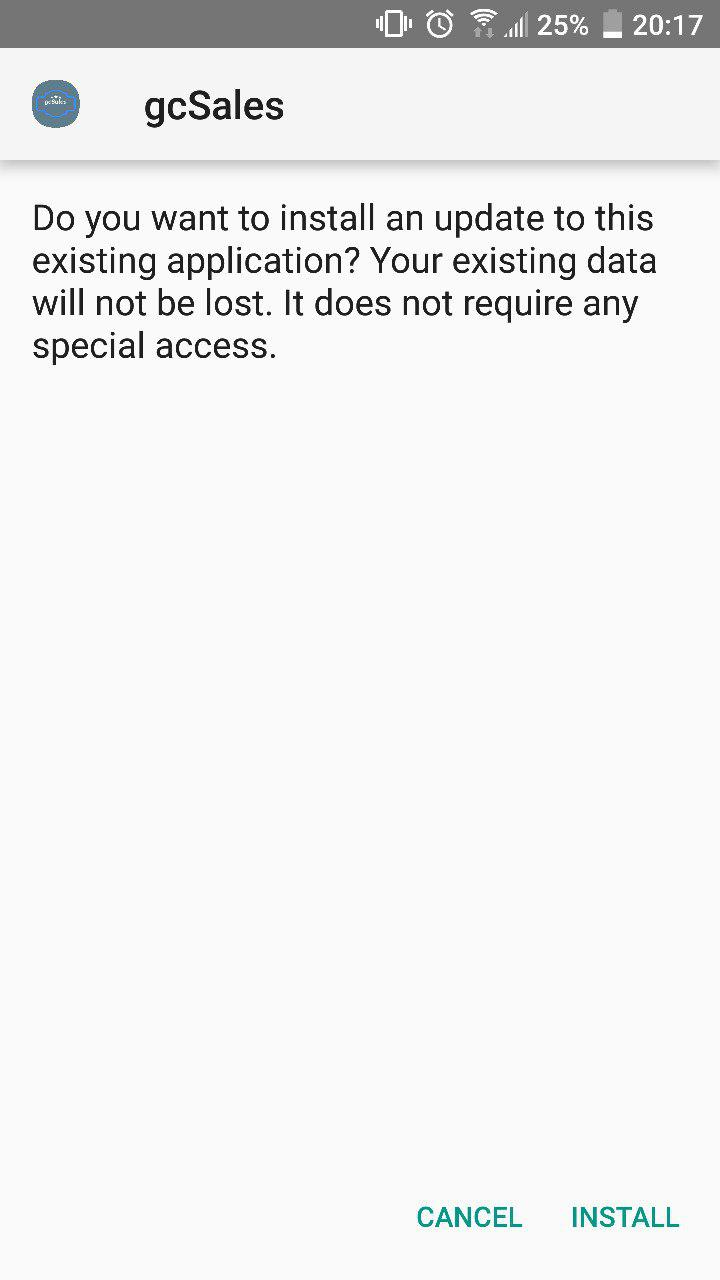
\includegraphics[height=0.38\textheight]{./screenshots/3/install_1.jpg}
    \caption{\small{начало установки}}
    \label{install1}
    \endminipage\hfill
    \minipage{0.3\textwidth}
    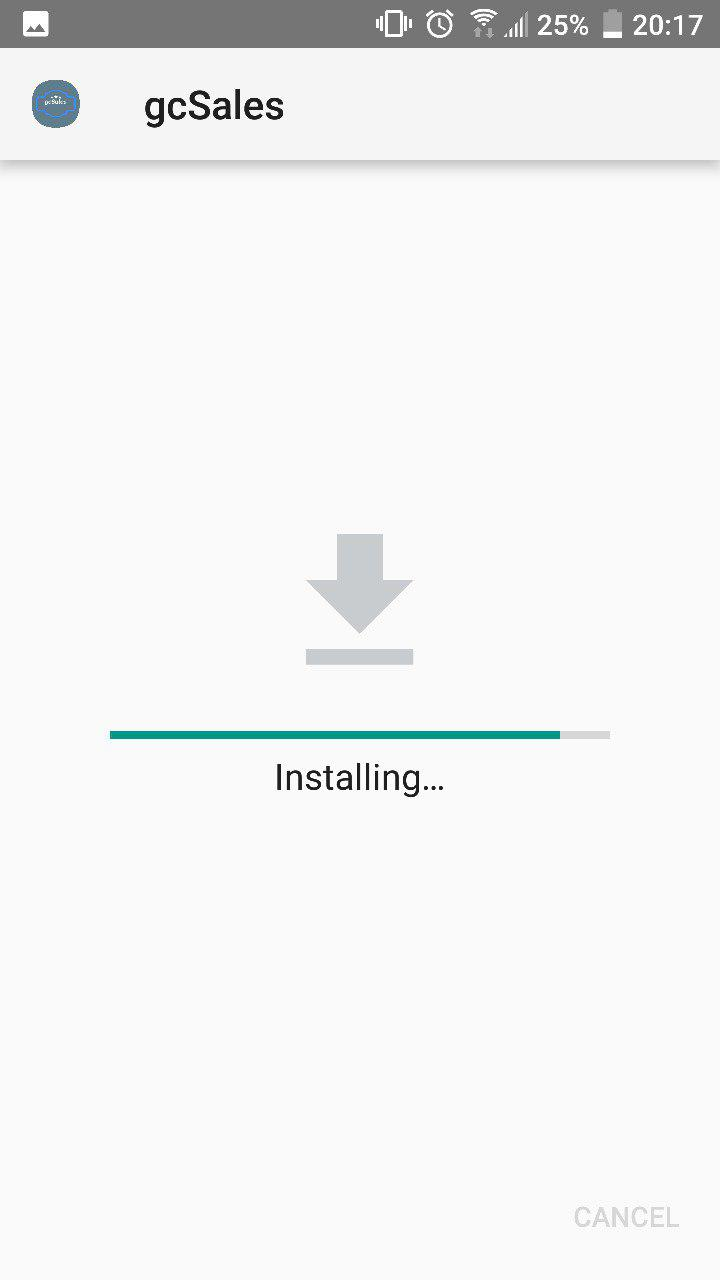
\includegraphics[height=0.38\textheight]{./screenshots/3/install_2.jpg}
    \caption{\small{процесс установки}}
    \label{install2}
    \endminipage\hfill
    \minipage{0.3\textwidth}
    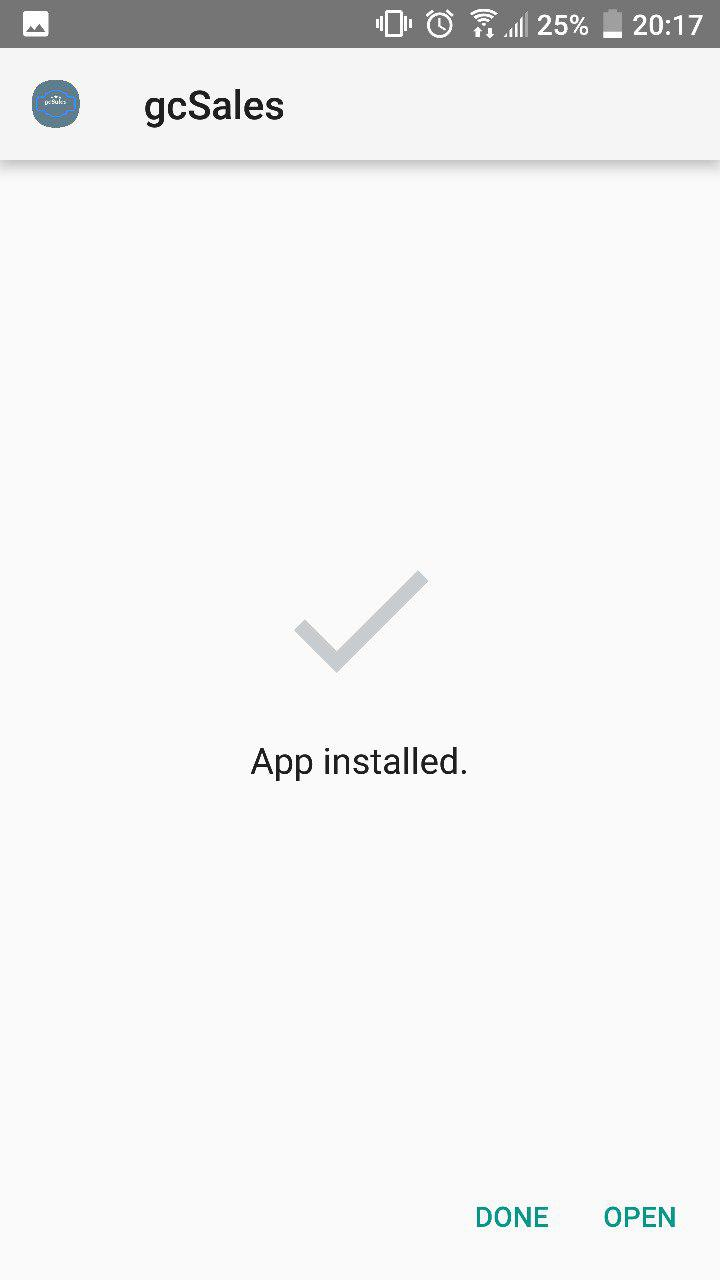
\includegraphics[height=0.38\textheight]{./screenshots/3/install_3.jpg}
    \caption{\small{приложение установлено}}
    \label{install3}
    \endminipage{}
\end{figure}


\subsubsection{Использование приложения}
Затем приложение необходимо открыть. Оператора будет приветствовать экран входа
в аккаунт. Есть возможность использовать приложение без входа и регистрации, но
при таком условии, оператору будут доступен ограниченный функционал, а именно
только просмотр акций. Регистрация даёт возможность работы со списками покупок.
(рис.~\ref{login},~\ref{register}).

\begin{figure}[h!]
    \centering
    \minipage{0.45\textwidth}
    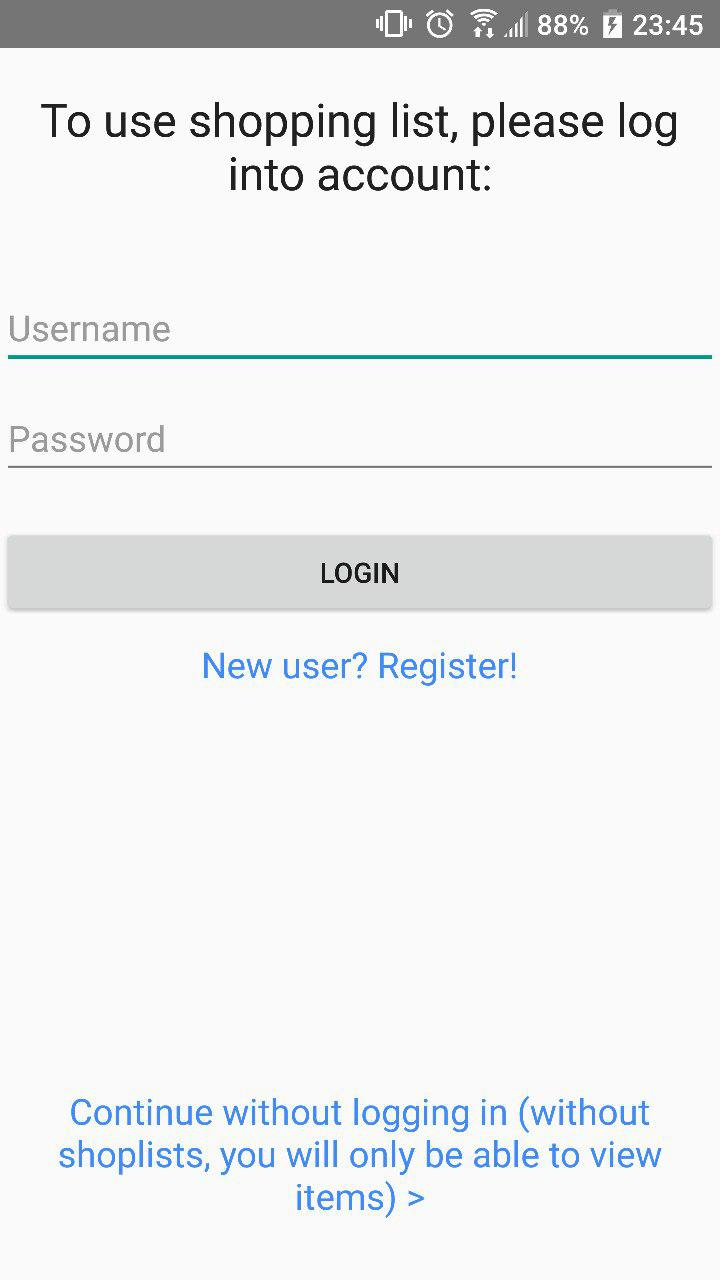
\includegraphics[height=0.37\textheight]{./screenshots/3/login.jpg}
    \caption{\small{вход в аккаунт}}
    \label{login}
    \endminipage\hfill
    \minipage{0.45\textwidth}
    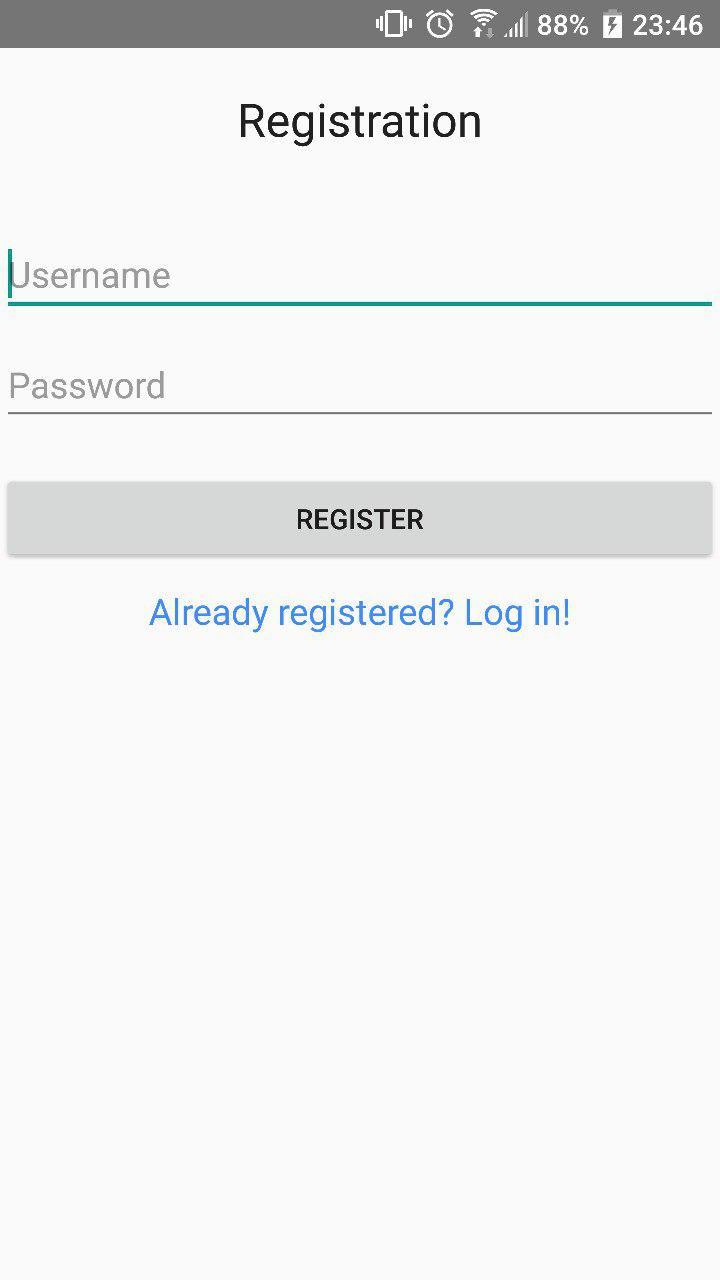
\includegraphics[height=0.37\textheight]{./screenshots/3/register.jpg}
    \caption{\small{регистрация аккаунта}}
    \label{register}
    \endminipage{}
\end{figure}

Войдя в аккаунт или выбрав режим без регистрации, пользователь попадает на
главный экран приложения (рис.~\ref{home}).

\begin{figure}[h!]
    \centering
    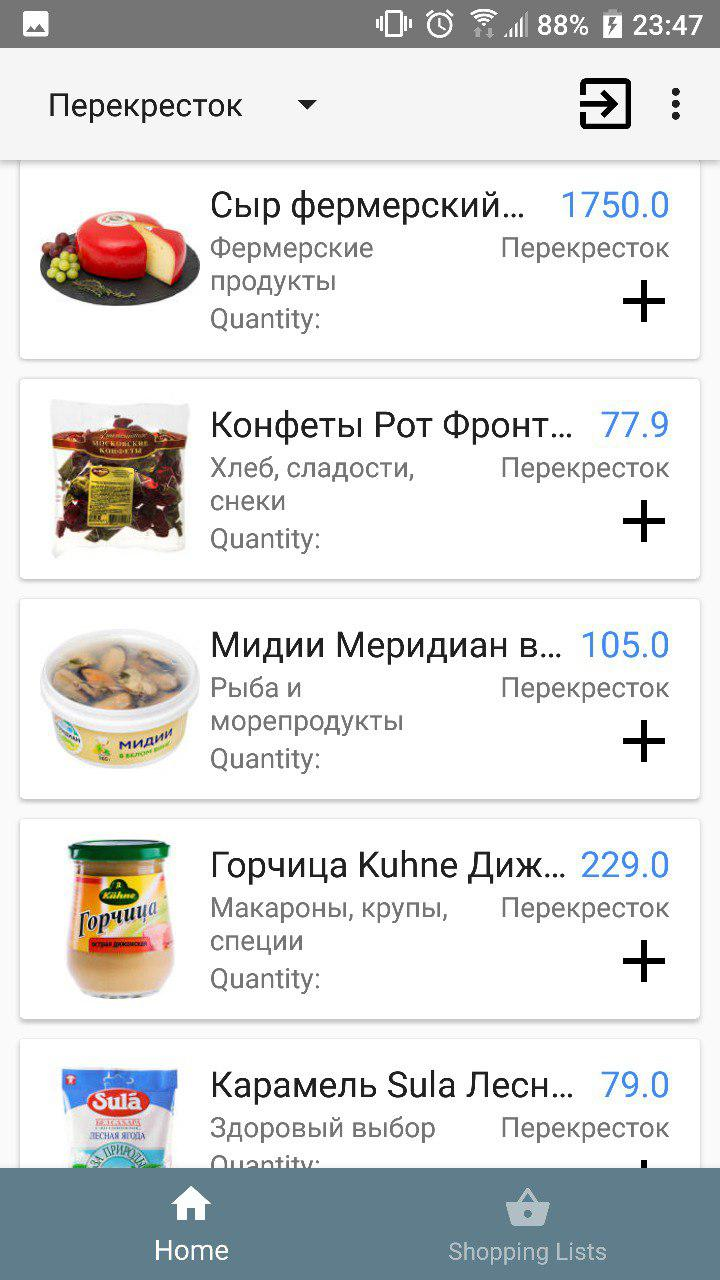
\includegraphics[height=0.35\textheight]{./screenshots/3/home.jpg}
    \caption{\small{просмотр всех акций}}
    \label{home}
\end{figure}

Далее, из любой активности оператор может вызвать раздел help (рис. \ref{help})
в меню приложения, где указана инструкция пользования данным продуктом. Также,
оператор имеет возможность просмотреть раздел about (рис. \ref{about}), где
написана общая информация о приложении и о разработчиках, и по долгому зажатию
на элементы button (кнопки), узнать её функционал (\ref{long_click}), что поможет ему лучше
разбираться в работе приложения.

\begin{figure}[h!]
    \centering
    \minipage{0.3\textwidth}
    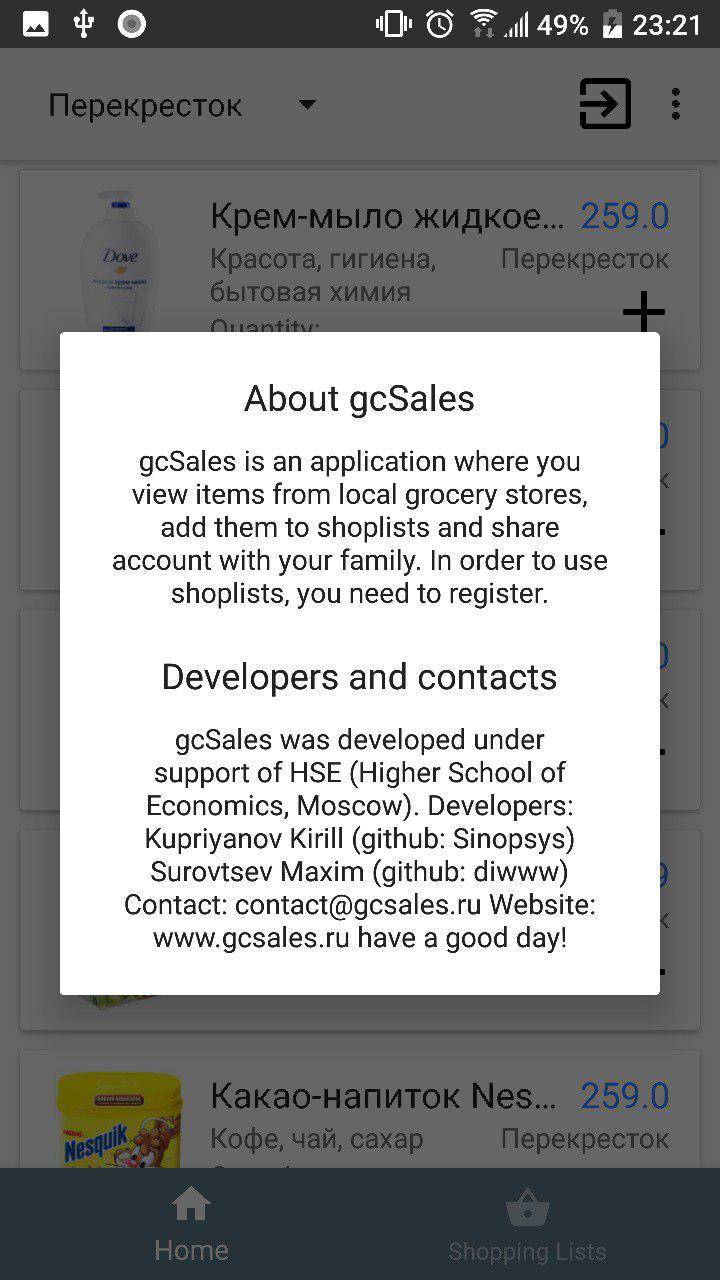
\includegraphics[height=0.35\textheight]{./screenshots/3/about.jpg}
    \caption{\small{просмотр раздела ``о приложении''}}
    \label{about}
    \endminipage\hfill
    \minipage{0.3\textwidth}
    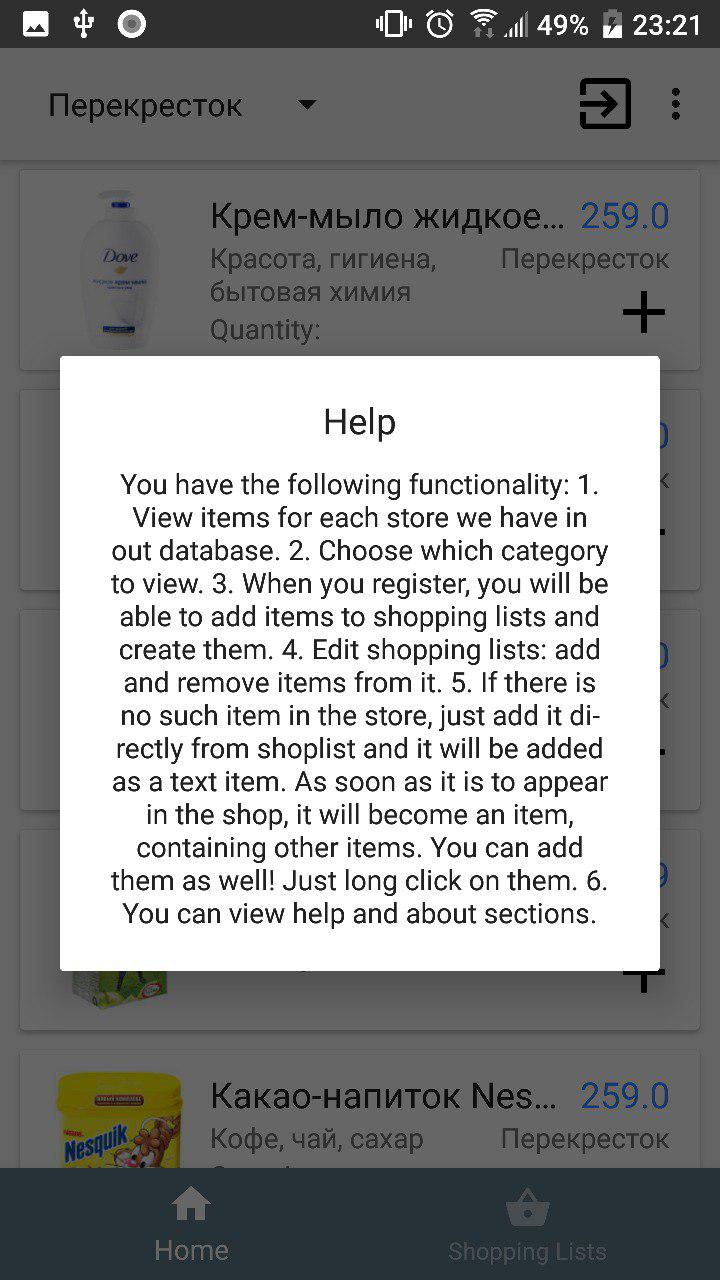
\includegraphics[height=0.35\textheight]{./screenshots/3/help.jpg}
    \caption{\small{просмотр подсказки пользования приложением}}
    \label{help}
    \endminipage\hfill
    \minipage{0.3\textwidth}
    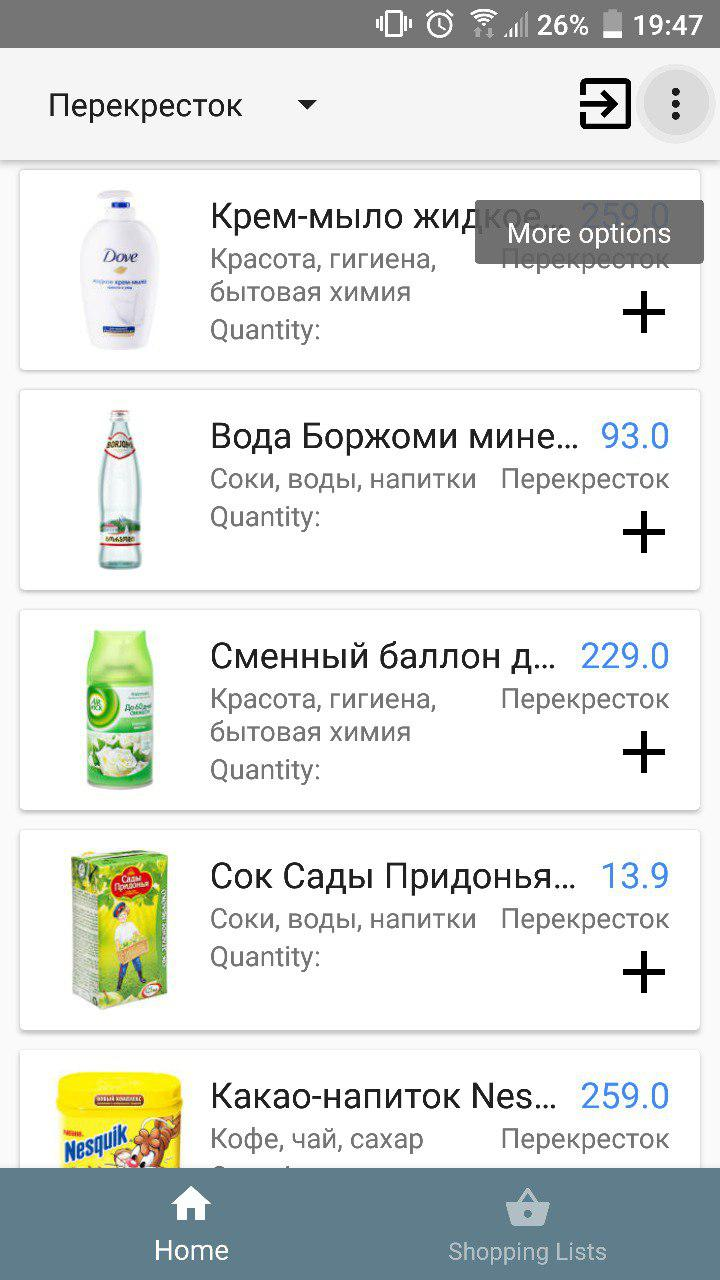
\includegraphics[height=0.35\textheight]{./screenshots/3/hint.jpg}
    \caption{\small{просмотр всплывающего описания элементов button (кнопок)}}
    \label{long_click}
    \endminipage{}
\end{figure}

\newpage



\newpage
\section{Приложение 1. Терминология}
\subsection{Терминология}
\begin{description}
  \item[REST (от англ. Representational State Transfer)] -- способ сетевого
    взаимодействия.  REST API определяет набор функций, к которым разработчики
    могут совершать запросы и получать ответы. Взаимодействие происходит по
    протоколу HTTP.  Преимуществом такого подхода является широкое
    распространение протокола HTTP, поэтому REST API можно использовать
    практически из любого языка программирования.
\end{description}



\newpage
\section{Приложение 2. Список используемой литературы}
\subsection{Список используемой литературы}
\begin{my_enumerate}
    \item
    ГОСТ 19.102-77 Стадии разработки. //Единая система программной документации. -М.: ИПК Издательство стандартов, 2001.
    
    \item
    ГОСТ 19.201-78 Техническое задание. Требования к содержанию и оформлению // Единая система программной документации. -М.:ИПК Издательство стандартов, 2001.
    
    \item  ГОСТ 19.404-79 Пояснительная записка. Требования к содержанию и оформлению. //Единая система программной документации. – М.: ИПК Издательство стандартов, 2001
    
    \item
    ГОСТ 19.101-77 Виды программ и программных документов
    //Единая система программной документации. -М.: ИПК Издательство стандартов, 2.: 001.
    
    \item
    ГОСТ 19.103-77 Обозначения программ и программных документов. //Единая система программной документации. -М.: ИПК Издательство стандартов, 2001.
    
    \item
    ГОСТ 19.104-78 Основные надписи //Единая система программной документации. -М.: ИПК Издательство стандартов, 2001.
    
    \item 
    ГОСТ 19.106-78 Требования к программным документам, выполненным печатным способом. //Единая
    система программной документации. – М.: ИПК Издательство стандартов, 2001
    
    \item 
    ГОСТ 19.603-78 Общие правила внесения изменений. //Единая система программной документации. –
    М.: ИПК Издательство стандартов, 2001
    
    \item
    Oculus Documentation [Электронный ресурс]: Режим доступа: https:// developer3.oculus. com/documentation/
    
    \item
    Oculus Developers Blog [Электронный ресурс]: chrispruett – Squeezing Performance out of your Unity Gear VR Game, 2015 - Режим доступа: https://developer3.oculus.com/blog /squeezing-performance-out-of-your-unity-gear-vr-game/
    
    \item 
    Uninty Scripting Reference [Электронный ресурс]: Режим доступа: https: //docs.unity3d. com/ScriptReference/
    
\end{my_enumerate}



% \newpage
%\section{Приложение 3. Изображение пользовательского интерфейса.}

% Index
\newpage
\eskdListOfChanges

% \phantomsection
% \addcontentsline{toc}{section}{Алфавитный указатель}
% \printindex

\end{document}
